\documentclass[%
  reprint,
  superscriptaddress,
  amsmath,amssymb,
  prl,
  floatfix,
  x11names
]{revtex4-2}

\usepackage{amsmath}
\usepackage{amssymb}
\usepackage{bm}
\usepackage{graphicx}
\usepackage{tikz}
\usetikzlibrary{arrows.meta,decorations.pathmorphing}
\usepackage{orcidlink}
\usepackage{hyperref}

\begin{document}

\title{Archimedean Resolution of the Bondi Runaway: \\
       Holes in a Background Substratum Gravitate Repulsively without Paradox}

\author{Karl Svozil\,\orcidlink{0000-0001-6554-2802}}
\email{karl.svozil@tuwien.ac.at}
\affiliation{Institute for Theoretical Physics, TU Wien, Wiedner Hauptstrasse 8-10/136, 1040 Vienna, Austria}

\date{\today}

\begin{abstract}
A localized absence of substratum in a positive-energy background acts, to leading order, as an effective negative-mass source whose pair dynamics with ordinary matter evades the Bondi runaway. A hole near a positive mass $M_+$ is pushed away from $M_+$ by Archimedean buoyancy in the substratum's infall, while $M_+$ is simultaneously repelled by the hole's negative effective source; both accelerations are aligned in the sense of mutual separation. No fundamental field violates the energy conditions: the apparent negativity is a background-subtraction artifact, structurally identical to Casimir energy, band-hole effective mass, and the peculiar gravity of cosmic voids.
\end{abstract}

\maketitle

\textit{Introduction.}---The negative-mass Schwarzschild solution has been regarded since Bondi~\cite{bondi-1957} as physically unrealizable. Treated as an autonomous point particle with intrinsic negative inertia, a negative mass placed near a positive one produces a runaway: the pair accelerates indefinitely in a common direction, conserving energy and momentum but violating dynamical stability. The standard energy conditions~\cite{hawking-ellis,wald-1984} forbid fundamental matter with $\rho<0$, reinforcing the view that repulsive solutions of the Einstein equations are mathematical curiosities.

We show that this conclusion does not survive once space is modeled as a \emph{background substratum}: a positive-energy-density medium $\rho_0>0$ whose local absence defines what we call a hole. The picture is an old one, going back to Einstein's 1920 reinterpretation of the gravitational ether~\cite{einstein-aether-en} and to Sakharov's induced gravity~\cite{Sakharov-67}, and it has a directly observed realization in cosmic voids~\cite{shethvdw-2004,hamaus-2014,nadathur-2019}. What is new here is a mechanical observation: in such a picture, the Bondi runaway is replaced by Archimedean mutual repulsion. The negative-mass degree of freedom is not autonomous; it is a buoyant displacement whose dynamics are set by the medium, and the medium's own gravitational response to a nearby positive mass drives the hole away from, not toward, that mass.

\textit{Setup.}---The substratum stress-energy $T^{(0)}_{\mu\nu}$ with $\rho_0>0$ is assumed to fill space outside the hole. For a Lorentz scalar, $T^{(0)}_{\mu\nu}=-\rho_0 g_{\mu\nu}$ ($p_0=-\rho_0$, equivalent to a cosmological constant $\Lambda=8\pi G\rho_0/c^2$); for a pressureless dust, $T^{(0)}_{\mu\nu}=\rho_0 u_\mu u_\nu$. Both choices support the central mechanism; the dust realization is empirically instantiated by cold dark matter on cosmological scales.

The hole occupies a bounded region $\Omega\subset\mathbb{R}^3$ in which $T_{\mu\nu}=0$. Only deviations from the uniform background source observable gravity; we define the background-subtracted effective stress-energy
\begin{equation}
T^{\text{eff}}_{\mu\nu}=T_{\mu\nu}-T^{(0)}_{\mu\nu},
\label{eq:Teff}
\end{equation}
which vanishes outside $\Omega$ and equals $-T^{(0)}_{\mu\nu}$ inside. The underlying field is positive everywhere; the negativity of $T^{\text{eff}}_{\mu\nu}$ in $\Omega$ is a renormalization, not a fundamental violation of the energy conditions.

\textit{Newtonian and linearized limit.}---In the weak-field limit, the shell theorem applied to $\rho^{\text{eff}}=-\rho_0\chi_\Omega$ yields a potential
\begin{equation}
\Phi(\mathbf{r})=\frac{G\rho_0 V(\Omega)}{r}+\mathcal{O}(\mathcal{R}^2/r^3)
\label{eq:phi}
\end{equation}
outside the bounding sphere $r=\mathcal{R}$ of $\Omega$, where $V(\Omega)$ is its Lebesgue measure. The leading field is positive and repels test bodies with an effective source
\begin{equation}
M_{\text{eff}}=-\rho_0 V(\Omega).
\label{eq:Meff}
\end{equation}
Equation~\eqref{eq:Meff} depends only on the volume of the absence: the shape of $\Omega$---spherical cavity, cubic cavity, foam, or fractal---enters only through subleading multipoles suppressed by $(\mathcal{R}/r)^2$. This shape-universality is exact in the linearized regime.

\textit{Exact exterior geometry.}---For a spherical hole in a Lorentz-scalar substratum, Birkhoff's theorem applies only to the source-free interior, which is therefore Minkowski. The exterior is not vacuum: it carries $T^{(0)}_{\mu\nu}\propto g_{\mu\nu}$, and the correct spherically symmetric solution is the Schwarzschild--de Sitter (Kottler) metric~\cite{kottler-1918},
\begin{equation}
F(r)=1-\frac{2GM_{\text{ext}}}{c^2 r}-\frac{\Lambda r^2}{3}.
\label{eq:SdS}
\end{equation}
Matching Minkowski interior to SdS exterior at $r=\mathcal{R}$ requires, by the Israel junction conditions~\cite{israel-1966,poisson-2004}, a thin boundary shell whose surface tension balances the bulk pressure jump $\Delta p=\rho_0$. The shell carries positive surface energy and ordinary tensile stress---not exotic matter. The asymptotic mass parameter is
\begin{equation}
M_{\text{ext}}=-\tfrac{4\pi}{3}\rho_0\mathcal{R}^3+M_{\text{shell}},
\end{equation}
and in the sub-cosmological regime $\Lambda\mathcal{R}^2\ll 1$ the bulk deficit dominates, $M_{\text{ext}}<0$, in agreement with Eq.~\eqref{eq:Meff}. Radial timelike geodesics in $F(r)$ accelerate outward: holes repel. For a dust substratum, the exterior is FLRW and the hole is a Lema\^{i}tre--Tolman--Bondi void~\cite{tolman-1934,bondi-1947}; no shell is needed and the boundary evolves smoothly.

\textit{Archimedean dynamics.}---We now turn to the main claim: the pair dynamics of a hole and a nearby positive mass $M_+$ does not exhibit the Bondi runaway. Let $\hat{\mathbf{n}}$ denote the unit vector from the hole's centroid toward $M_+$, and let $r$ be their separation.

Two effects operate simultaneously (Fig.~\ref{fig:archimedes}). The positive mass, treated as a test body in the hole's exterior field Eq.~\eqref{eq:SdS}, experiences a gravitational acceleration directed away from the hole,
\begin{equation}
\mathbf{a}_{M_+}=+\frac{G|M_{\text{ext}}|}{r^2}\,\hat{\mathbf{n}},
\label{eq:aMplus}
\end{equation}
with the $+\hat{\mathbf{n}}$ sign inherited from $M_{\text{ext}}<0$. Independently, the substratum surrounding the hole is itself pulled toward $M_+$ by ordinary gravitational attraction, acquiring an acceleration $\mathbf{g}_{\text{at hole}}(M_+)=+(GM_+/r^2)\hat{\mathbf{n}}$ at the hole's location. The hole, being the \emph{absence} of substratum within a flowing medium, is Archimedean: its acceleration is opposite to that of the displaced fluid,
\begin{equation}
\mathbf{a}_{\text{hole}}=-\mathbf{g}_{\text{at hole}}(M_+)=-\frac{GM_+}{r^2}\,\hat{\mathbf{n}}.
\label{eq:ahole}
\end{equation}
The positive mass accelerates along $+\hat{\mathbf{n}}$ (away from the hole), the hole along $-\hat{\mathbf{n}}$ (away from $M_+$). Both objects accelerate \emph{away from each other}. The pair separates; there is no runaway.

\begin{figure}[b]
\centering
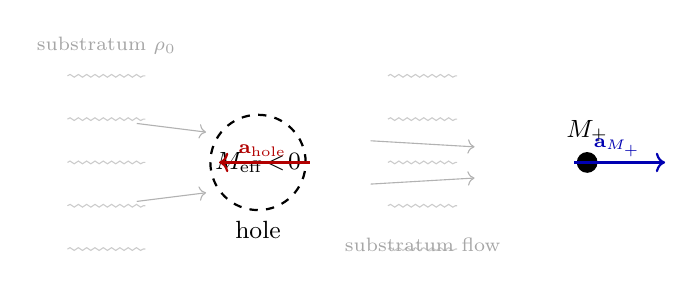
\begin{tikzpicture}[scale=1.1]
% hole (dashed circle with interior minus sign)
\draw[thick,dashed] (0,0) circle (0.55);
\node at (0,0) {\small $M_{\text{eff}}\!<\!0$};
\node[below=0.02cm] at (0,-0.55) {\small hole};
% substratum indication - wavy background on one side
\foreach \y in {-1.0,-0.5,0,0.5,1.0}{
  \draw[gray!40, decorate, decoration={snake, amplitude=0.5pt, segment length=3pt}]
    (-2.2,\y) -- (-1.3,\y);
  \draw[gray!40, decorate, decoration={snake, amplitude=0.5pt, segment length=3pt}]
    (1.5,\y) -- (2.3,\y);
}
\node[gray!70] at (-1.75,1.35) {\scriptsize substratum $\rho_0$};
% positive mass
\fill (3.8,0) circle (0.12);
\node[above] at (3.8,0.12) {\small $M_+$};
% arrows
\draw[->,thick,red!70!black] (0.6,0.0) -- (-0.45,0.0);
\node[red!70!black, above=-0.05cm] at (0.05,0.0) {\scriptsize $\mathbf{a}_{\text{hole}}$};
\draw[->,thick,blue!70!black] (3.65,0.0) -- (4.7,0.0);
\node[blue!70!black, above=-0.05cm] at (4.15,0.0) {\scriptsize $\mathbf{a}_{M_+}$};
% flow arrows showing substratum moving toward M_+
\draw[->, gray!60, thin] (-1.4,0.45) -- (-0.6,0.35);
\draw[->, gray!60, thin] (-1.4,-0.45) -- (-0.6,-0.35);
\draw[->, gray!60, thin] (1.3,0.25) -- (2.5,0.18);
\draw[->, gray!60, thin] (1.3,-0.25) -- (2.5,-0.18);
\node[gray!70] at (1.9,-0.95) {\scriptsize substratum flow};
\end{tikzpicture}
\caption{Archimedean repulsion. The substratum (wavy background) flows gravitationally toward $M_+$; the hole, as a buoyant absence, is displaced in the opposite direction, $\mathbf{a}_{\text{hole}}$ [Eq.~\eqref{eq:ahole}]. Simultaneously, $M_+$ is gravitationally repelled by the hole's effective negative source, $\mathbf{a}_{M_+}$ [Eq.~\eqref{eq:aMplus}]. Both accelerations point away from the other body, producing mutual repulsion rather than Bondi pair runaway.}
\label{fig:archimedes}
\end{figure}

Two features distinguish this from Bondi's analysis. First, the hole has no intrinsic inertia. Its dynamical response is inherited entirely from the surrounding substratum and follows from Archimedes' principle applied to a non-uniform acceleration field. The paradoxical ``chasing'' behavior that Bondi derived requires treating the negative-mass object as an autonomous Newtonian particle with $m<0$; the hole is not such an object. Second, the sign of $\mathbf{a}_{\text{hole}}$ is fixed by fluid kinematics, not by $M_{\text{ext}}$: it would be the same for any substratum flow directed toward $M_+$, regardless of what the hole's effective gravitational charge might be. Momentum conservation is respected, with the missing momentum supplied by the substratum's gravitational response to $M_+$; the medium, not the hole, is the reservoir.

The same mechanism governs well-known non-gravitational analogues. A semiconductor hole subjected to an electric field accelerates with the sign appropriate to negative effective mass, but no runaway instability arises because the underlying electrons, all of positive mass, obey ordinary dynamics within the adiabatic band~\cite{kittel-ssp,ashcroft-mermin}. Dirac's hole-theoretic positron~\cite{dirac-1930} is the relativistic analogue of the same construction. The present result is the gravitational analogue.

\textit{Energy conditions.}---The fundamental stress-energy $T_{\mu\nu}$ is nowhere negative. Inside the hole $T_{\mu\nu}=0$, outside $T_{\mu\nu}=T^{(0)}_{\mu\nu}$ with $\rho_0>0$. The Lorentz-scalar realization has $p_0=-\rho_0$ and thereby violates the strong energy condition---but in exactly the same sense and to the same degree as the cosmological-constant component driving the observed cosmic acceleration~\cite{Riess1998,Perlmutter1999}, a violation universally accepted as empirically required. The dust realization satisfies all standard energy conditions. Negativity enters only in the bookkeeping object $T^{\text{eff}}_{\mu\nu}$ of Eq.~\eqref{eq:Teff}, constructed to isolate the local gravitational effect of the deviation from baseline. This is the same structural move that renders the Casimir energy negative~\cite{casimir-1948,milton-2001}, the band hole's inertial mass effectively negative~\cite{kittel-ssp}, and the peculiar gravity of a cosmic void repulsive~\cite{shethvdw-2004,hamaus-2014}. In none of these cases does the negativity of the subtracted quantity signal a pathology of the underlying theory.

\textit{Discussion.}---The result is narrow but sharp. Within a background-substratum framework, gravitational repulsion between an underdense region and ordinary matter is generic, the Bondi pair-runaway objection does not apply, and the standard energy conditions of the fundamental field are preserved. What the framework does \emph{not} establish is the existence of such a substratum on sub-cosmological scales, which remains a hypothesis. The closest empirical realization is cosmic void cosmology, in which the dust-like substratum is simply cold dark matter and the repulsive peculiar gravity of voids relative to the cosmic mean is an observed phenomenon, measured through redshift-space distortions in the void-galaxy cross-correlation and other probes~\cite{hamaus-2014,nadathur-2019}.

The Archimedean mechanism suggests where to look for a compact-object realization. A candidate signature is a localized object of negative gravitational charge whose trajectory tracks, at leading order, the negative gradient of the Newtonian potential produced by surrounding matter---opposite to the trajectory of an ordinary self-gravitating body. For such an object, lensing is defocusing, Shapiro delays become advances, and orbital dynamics are inverted. None has been detected at sub-cosmological scales, and the framework presented here is consistent with that null result: it predicts only that \emph{if} a ponderable substratum exists and \emph{if} it admits localized absences on astrophysical scales, such signatures should appear. The framework moves the question from ``can negative-mass sources exist at all'' to ``does a substratum exist in which they can be realized as absences,'' which is an empirical question we do not claim to settle.

\textit{Conclusion.}---The Bondi runaway is an artifact of treating a negative-mass source as an autonomous dynamical particle. In a substratum picture, the negative effective source is a buoyant absence with no intrinsic inertia, and its dynamics, set by the surrounding medium, produce mutual repulsion with any nearby positive mass rather than runaway pursuit. The result requires neither exotic fundamental matter nor violation of the underlying energy conditions, and it places gravitational repulsion conceptually alongside Casimir energy, band holes, and void peculiar gravity---familiar, unexotic consequences of background subtraction in a positive-energy medium.

\begin{acknowledgments}
The author thanks an anonymous referee of an earlier version for incisive criticism concerning the non-vacuum exterior, the Israel junction conditions, the substratum equation of state, and the Archimedean mechanism itself. This text was partially created and revised with assistance from large language models; all content, ideas, and prompts were provided by the author. This research was funded in whole or in part by the Austrian Science Fund (FWF) Grant DOI: 10.55776/PIN5424624. The author acknowledges TU Wien Bibliothek for financial support through its Open Access Funding Programme.
\end{acknowledgments}

\bibliography{svozil}

\end{document}
